\documentclass{article}
\usepackage{graphicx}
\usepackage{color}

\sloppy
\definecolor{lightgray}{gray}{0.5}
\setlength{\parindent}{0pt}

\title{UPENN \\937 \\ Problem Set 03\\ }
\author{Rodrigo A. Morales M.}
\date{27. dic. 2018}

\begin{document}

\maketitle

\begin{center}
   \includegraphics[scale=0.05]{logo1.png}
\end{center}

    
    
\subsection*{Contents}



\begin{itemize}
\setlength{\itemsep}{-1ex}
   \item Part I. Familiarize with the code.
   \item The model.
   \item Parameters.
   \item 1.c) What do you learn from the output of sim\textunderscore stationary()?
   \item 1.e) Changes required to run for a tighter constraint.
   \item Part II, new Constraint.
   \item 2.a) Interpretation.
   \item 2.b) New Steady State.
   \item 2.c) Rewrite constraint.
   \item 2.d) New Version of the code.
   \item 2.e) Numerical solution.
   \item 2.f) Main economic effects.
   \item Extra: 1.c) Output of sim\textunderscore stationary()
\end{itemize}


\subsection*{UPENN, 937, Prof. Tim Landvoigt, Problem set 03.}

\begin{par}
Rodrigo Morales Mendoza, Dec. 2019
\end{par} \vspace{1em}


\subsection*{Part I. Familiarize with the code}

The readmfe file explains the usage of the code. Basically, there are three ``main'' modules:

\begin{itemize}
	\item main\textunderscore setup() sets the model parameters and experiments. It also computes the steady state and generates the first objects with guesses for the Value Function and state space matrices, which are used for the convergence algorithm. The main inputs are: the experdef() module that defines the parameters, the type of experiment to be run (benchmark is the default), the data to load if pre-existing one is to be used, and whether or not to compute the analytical jacobian. The main output is the `env\textunderscore$\{experiment\}$.mat' data, which will be used for the next routines. 
	\item main\textunderscore execute(), iterates to solve the equations. The main output is `res\textunderscore\{date\}.mat', which contains the value and policy functions when the algorithm converges.
	\item sim\textunderscore stationary(), simulates the economy for many periods and computes the moments of the variables, while also calculating the Euler equation errors along the simulated path. Main output is the data that will be used for the sim\textunderscore trans().
	\item sim\textunderscore trans(), computes the impulse response functions or transition dynamics, first reading the ergodic distribution computed previously and then initializes the simulation of many short model paths. It simulates these paths for different initial exogenous productivity states.
	\item plot\textunderscore trans() reads the previous matrix result and does the plots, saving them as well in the hard disk.
\end{itemize}

\subsection*{The model}

The basic equations of the KM model are divided into the farmer and the gatherer.

Farmer:

$$ V^F(z,w) = \max_{c,k^{\prime},b^{\prime} } \left( u(c) + \beta_F E_z \left[ V(z^{\prime},w^{\prime} \right]  \right) $$

$$ \textsc{s.t.} \quad \quad c+qk^\prime+b^\prime = ak + qk +Rb - \phi(k^\prime/k - 1)^2k/2$$
$$-b^\prime \leq \theta qk^\prime $$

which gives the following equilibrium conditions (after FOCs):

\begin{eqnarray*}
 q & = & \beta_F E_z\left[ \frac{u^\prime(c^\prime)}{u^\prime(c)}(a+q+\frac{\phi((k^\prime/k)^2 -1)}{2})\right]+\mu \theta q\\
 1 & = & \mu + \beta_F E_z\left[R\frac{u^\prime(c^\prime)}{u^\prime(c)}\right] \\
 0 & = & \mu (\theta q k^\prime + b^\prime) 
\end{eqnarray*}

Gatherer:

$$ V^G(z,w) = \max_{c,k^{\prime},b^{\prime} } \left( u(c) + \beta_G E_z \left[ V(z^{\prime},w^{\prime} \right]  \right) $$

$$ \textsc{s.t.} \quad \quad c+qk^\prime+b^\prime = G(k) + qk +Rb$$

which gives the following equilibrium conditions (after FOCs):

\begin{eqnarray*}
 q & = & \beta_G E_z\left[ \frac{u^\prime(c^\prime)}{u^\prime(c)}\left(G^\prime(k^\prime)+q\right)\right]\\
 1 & = & \beta_G E_z\left[R\frac{u^\prime(c^\prime)}{u^\prime(c)}\right]
\end{eqnarray*}


\subsection*{Parameters}


\begin{verbatim}
params.a=1;
params.alower=.9;
params.sig_a=.01;
%params.sig_a=.0001;
params.rho_a=0.5;
params.N_a=5; % Number of discrete states

% preferences
params.gamma=2;
params.betaF=0.95;
params.betaG=0.98;

% technology
params.alpha=0.7;
params.Kbar=1;
params.phi=0;

% credit
params.theta=0.9;
params.use_min_q = false;
\end{verbatim}


\subsection*{1.c) What do you learn from the output of sim\textunderscore stationary()}

I include the output of sim\textunderscore stationary() in the end of this document.

We learn from this output many things:

\begin{itemize}
	\item Checking that the min/max of the endogenous state variables are within the boundaries set for their grids ex-ante.
	\item Evaluating the main moments of the functional equation errors.
	\item Checking that $\lambda = 0$ throughout the exercise.
	\item Also, it allows to compare simulated moments across experiments to examine impact of parameter change.
\end{itemize}

All seems to be working fine with respect to these regards.

\subsection*{1.e) Changes required to run for a tighter constraint.}

\begin{itemize}
	\item Generate a new \{`theta08'\} grid definition in the program `experdef.m', as well as its corresponding endogenous grid if required.
	\item In general, the main programs will generate output of data which will change from run to run, so it will be required to use the appropriate name, as in any usual run of the code.
\end{itemize}


\subsection*{Part II, New constraint}

$$b_{t+1}^F \leq \theta \left( a(x_{t+1}) + q(x_{t+1}) \right)k_{t+1}^F  \quad \quad \quad \forall x_{t+1} \in X_{t+1} $$


The equations do not change for the gatherer, and the Farmer will be facing a very similar problem, with the following equations (the only change comes from the constraint):

Farmer:

$$ V^F(z,w) = \max_{c,k^{\prime},b^{\prime} } \left( u(c) + \beta_F E_z \left[ V(z^{\prime},w^{\prime} \right]  \right) $$

$$ \textsc{s.t.} \quad \quad c+qk^\prime+b^\prime = ak + qk +Rb - \phi(k^\prime/k - 1)^2k/2$$
$$b^\prime \leq \theta \left( a^\prime + q^\prime \right)k^\prime $$

which gives the following equilibrium conditions (after FOCs):

\begin{eqnarray*}
 q & = & \beta_F E_z\left[ \frac{u^\prime(c^\prime)}{u^\prime(c)}(a+q+\frac{\phi((k^\prime/k)^2 -1)}{2})\right]+\mu \theta (a^\prime + q^\prime)\\
 1 & = & \mu + \beta_F E_z\left[R\frac{u^\prime(c^\prime)}{u^\prime(c)}\right] \\
 0 & = & \mu \left[\theta (a^\prime + q^\prime) k^\prime + b^\prime\right] 
\end{eqnarray*}


\subsection*{2.a) Interpretation.}

The borrowing constraint now depends on a fraction of the minimum capital wealth of tomorrow. The intuition is as follows.

The interpretation of this new constraint is basically a protection for the lender (gatherer): it prevents the borrower (farmer) to not be able to pay its debt fully on the next period without needing to ask for even more money, which is more likely to be binding in the cases where the shock the next period is low. That is why if the restriction is precisely fixed for the lowest state possible, then it assures that it will always be binding for any other case.
    

\subsection*{2.b) New Steady State.}

Again, the steady state is very similar as the previous case, with a few modifications, namely:

\begin{eqnarray*}
  \mu_F & = & 1-\beta_F/\beta_G  \\
  q & = & \frac{\beta_F a + \theta a\mu_F}{1-\beta_F - \theta\mu_F}   \\
  k_{F,ss} & = & \left[ \frac{\alpha \underline{a}(1-\beta_F - \theta\mu_F)\beta_G)}{(1-\beta_G) a (\beta_F + \theta \mu_F)} \right]^{\frac{1}{1-\alpha}}  \\
  b_F & = & -\theta(q + a) k_{F,ss}
\end{eqnarray*}


\subsection*{2.c) Rewrite constraint.}

Using the minimum of (q+a) at any given time is enough, as that guarantees that it will always be binding (if it is binding for the lowest state). The code already has an implementation for such variable, which needs to be indicated in the `experdef' file, and needs to add $min(q+a))$ in the `calcEquations' files.


%\subsection*{2.d) New Version of the code.}


%\subsection*{2.e) Numerical solution.}


\subsection*{2.f) Main economic effects.}







%PLOT OF IRFs
\begin{figure}
\caption{IRFs 1 for unmodified code:}
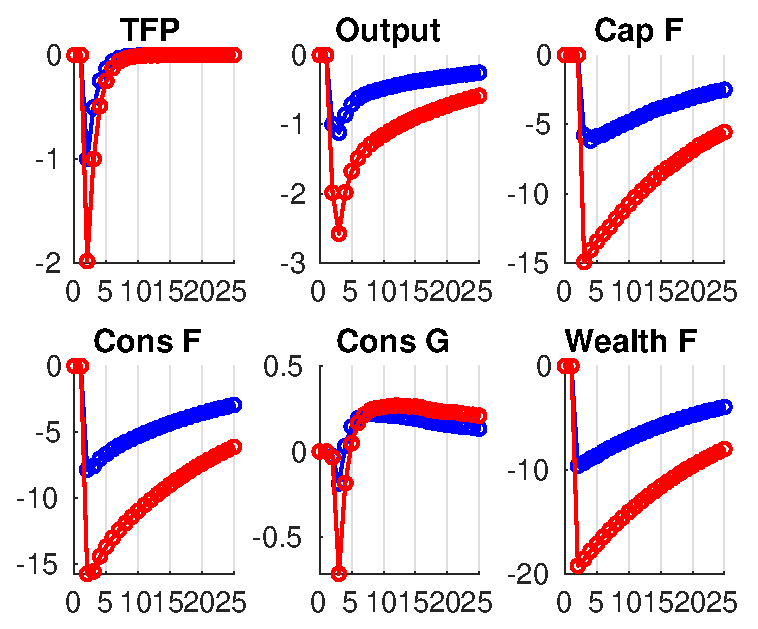
\includegraphics [width=5in]{PS03_projection_code_modif/Results/GR_orig_diff_IRF1.eps}
\end{figure}

\begin{figure}
\caption{IRFs 2 for unmodified code:}
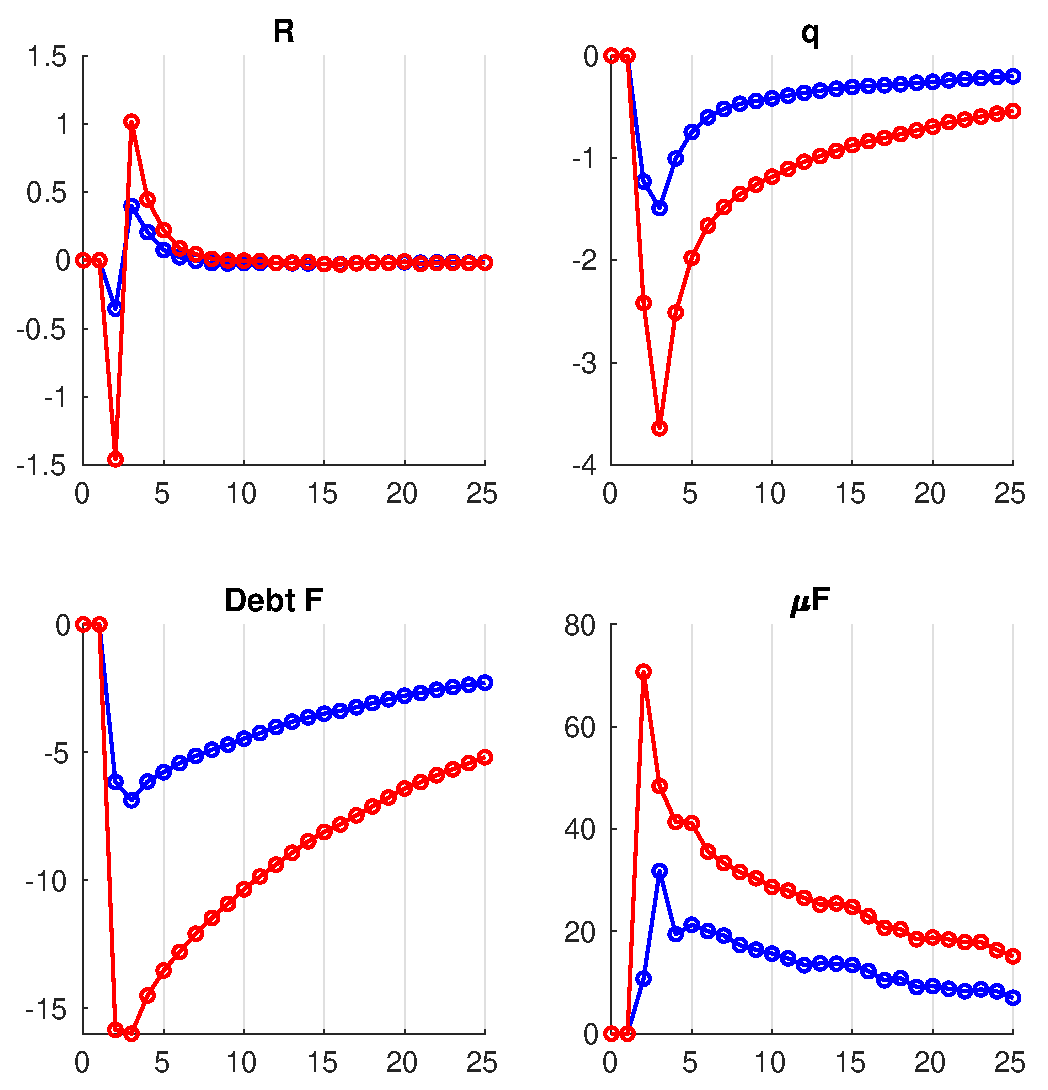
\includegraphics [width=4in]{PS03_projection_code_modif/Results/GR_orig_diff_IRF2.eps}
\end{figure}



\subsection*{Extra: 1.c) Output of sim\textunderscore stationary()}


\color{lightgray} \begin{verbatim} 
Simulation steady state
Frequency (exog subsamples): 9999.000000	3162.000000	6838.000000	
-------------
5	   R					1.020408 |	1.019113, 0.010460 |	1.017850, 0.009993 |	1.019696, 0.010619 |
22	   Y					1.077365 |	1.071265, 0.027937 |	1.089912, 0.020631 |	1.062644, 0.026635 |
1	   a					0.000000 |	0.999986, 0.010115 |	1.012053, 0.004091 |	0.994407, 0.006587 |
2	alower					0.000000 |	0.899988, 0.009103 |	0.910848, 0.003682 |	0.894966, 0.005928 |
17	bFpol					-23.657270 |	-23.108187, 4.968757 |	-25.664515, 3.446048 |	-21.926226, 5.117933 |
18	bGpol					23.657270 |	23.109600, 4.969037 |	25.666051, 3.446298 |	21.927583, 5.118211 |
28	bind_muF				0.000000 |	0.595960, 0.490730 |	0.318786, 0.466079 |	0.724188, 0.446955 |
13	  cF					0.138347 |	0.132895, 0.031842 |	0.150491, 0.029638 |	0.124758, 0.029448 |
14	  cG					0.939018 |	0.937553, 0.015172 |	0.938495, 0.016943 |	0.937120, 0.014259 |
30	eff_theta				0.000000 |	1.000000, 0.000000 |	1.000000, 0.000000 |	1.000000, 0.000000 |
25	expRF					0.000000 |	1.024116, 0.010650 |	1.021603, 0.012210 |	1.025277, 0.009626 |
26	expRG					0.000000 |	1.020635, 0.010363 |	1.019118, 0.011013 |	1.021336, 0.009971 |
20	  kF					0.621148 |	0.613308, 0.126437 |	0.645528, 0.111327 |	0.598413, 0.130174 |
16	kFpol					0.000000 |	0.613309, 0.126437 |	0.675182, 0.089967 |	0.584697, 0.130560 |
19	kGpol					0.378852 |	0.383105, 0.125320 |	0.322087, 0.088084 |	0.411320, 0.129849 |
11	lamF					0.000000 |	0.000000, 0.000000 |	0.000000, 0.000000 |	0.000000, 0.000000 |
12	lamG					0.000000 |	0.000000, 0.000000 |	0.000000, 0.000000 |	0.000000, 0.000000 |
21	levF					0.918367 |	0.909176, 0.018263 |	0.896154, 0.017104 |	0.915199, 0.015421 |
27	min_q					0.000000 |	41.878414, 1.397808 |	42.794101, 1.003619 |	41.455119, 1.350798 |
10	 muF					0.312823 |	0.374079, 0.319417 |	0.176181, 0.270559 |	0.465628, 0.298109 |
15	   q					42.318182 |	41.882492, 1.396205 |	42.797771, 1.002475 |	41.459386, 1.348953 |
24	  wF					2.766932 |	3.004526, 0.986415 |	3.562434, 0.948822 |	2.746503, 0.892256 |
29	wFsh					0.000000 |	0.071315, 0.022584 |	0.083092, 0.022060 |	0.065869, 0.020666 |
23	  wG					40.628614 |	39.945153, 1.112652 |	40.321578, 1.103282 |	39.771260, 1.073325 |
 
-----------------------------------------------
Average and maximum Euler equation error
Equ.no.		Avg.		Med.		p75			p95			p99			p99.5		Max.
1			0.001541	0.000979	0.002491	0.004519	0.005377	0.005652	0.006113
2			0.000175	0.000171	0.000241	0.000375	0.000524	0.000569	0.001899
3			0.001213	0.001023	0.001996	0.003319	0.004137	0.004191	0.004243
4			0.000370	0.000281	0.000524	0.000737	0.000866	0.000946	0.001654
5			0.013666	0.010426	0.019042	0.026615	0.030742	0.034392	0.057525
6			0.003060	0.001425	0.003268	0.011584	0.012153	0.012197	0.012236
7			0.005550	0.005243	0.009094	0.014481	0.017767	0.018044	0.018344
8			0.001413	0.001395	0.001890	0.002309	0.002383	0.002390	0.002417
9			0.003586	0.003065	0.005949	0.009904	0.012224	0.012421	0.012616
10			0.000894	0.000414	0.001459	0.002942	0.003465	0.003636	0.003932
State bounds:
    0.0600    0.7500
    0.8000    1.0000

Simulation mins:
    0.1387    0.7916

Simulation max:
    0.7639    0.9526

Saving simulation data to .mat file: sim_res_01.mat
\end{verbatim} \color{black}


% Include table of values for kappa (standard):
%\begin{center}
%\begin{tabular}{llll}
%Y & K & Cons & IntegralV \\ 
%\hline 
%1.6919 & 6.4066 & 1.1793 & -0.59333 \\ 
%\hline 
%\end{tabular}
%\end{center}


%\vspace{1em}
%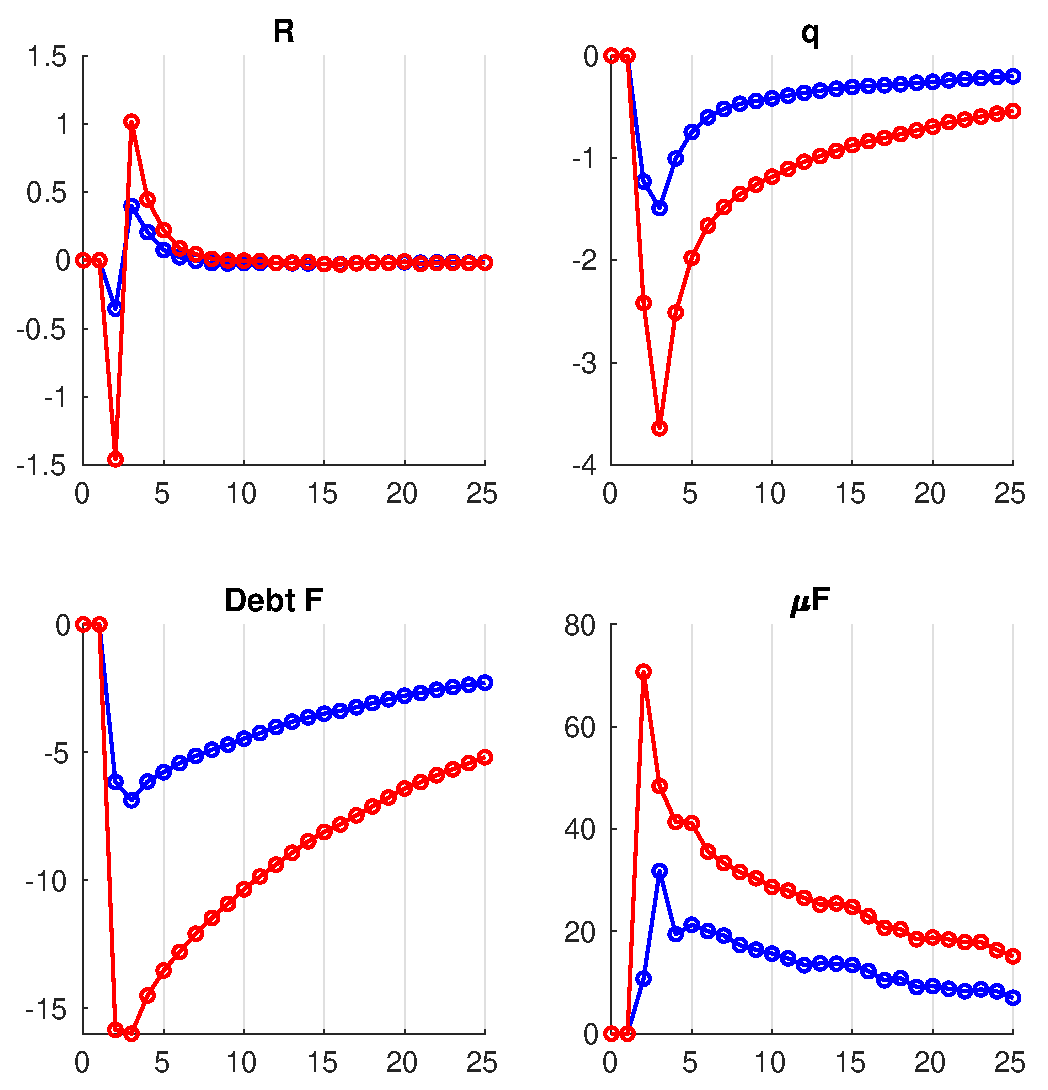
\includegraphics [width=4in]{PS03_projection_code_modif/Results/GR_orig_diff_IRF2.eps}

\end{document}
